Escribe el grupo (familia), el período y el tipo de clasificación de los siguientes elementos. Después de realizar este ejercicio, ubica a cada elemento en la tabla
% periódica que se muestra abajo.
\renewcommand{\arraystretch}{1.5}

% \begin{minipage}{.40\textwidth}
\begin{table}[H]
    \centering
    \begin{tabular}{r|>{\centering\columncolor{DarkOliveGreen!10}}p{2.2cm}>{\centering\columncolor{Sepia!10}}p{1.1cm}p{1.2cm}}
        Elemento & Grupo/Familia & Período & Tipo \\    \hline
        % Plata   &              &         &       \\    \hline
        % Bario   &              &         &       \\    \hline
        % Potasio  &              &         &      \\    \hline
        % Niquel  &              &         &       \\    \hline
        % Yodo     &              &         &      \\    \hline
        Paladio  &               &         &      \\    \hline
        Oro      &               &         &      \\    \hline
        Argón    &               &         &      \\    \hline
        Samario  &               &         &      \\    \hline
        Talio    &               &         &      \\    \hline
    \end{tabular}
\end{table}
% \end{minipage}\hfill
% \begin{minipage}{.5\textwidth}
%     \begin{figure}[H]
%         \centering
%         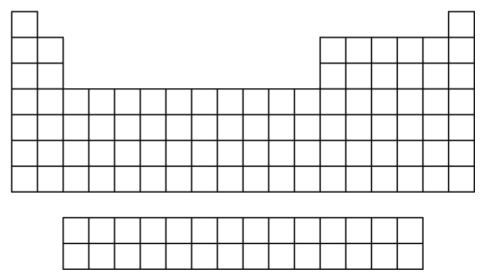
\includegraphics[width=\linewidth]{../images/blank-periodictable}
%     \end{figure}
% \end{minipage}
